\documentclass[../main/report.tex]{subfiles}
\begin{document}

\section{Backup oriented design}

Verifying a PCB design is difficult.
If the circuitry has been designed incorrectly, there may not be much that can be done, except for designing a new PCB.
Because of this, the PCB has backup solutions for all major components, and exposes as much as possible of the important circuitry on headers.
This enables us to probe signals for debugging purposes, and also do manual rewiring in case of faulty wiring.

\begin{figure}[H]
    \centering
    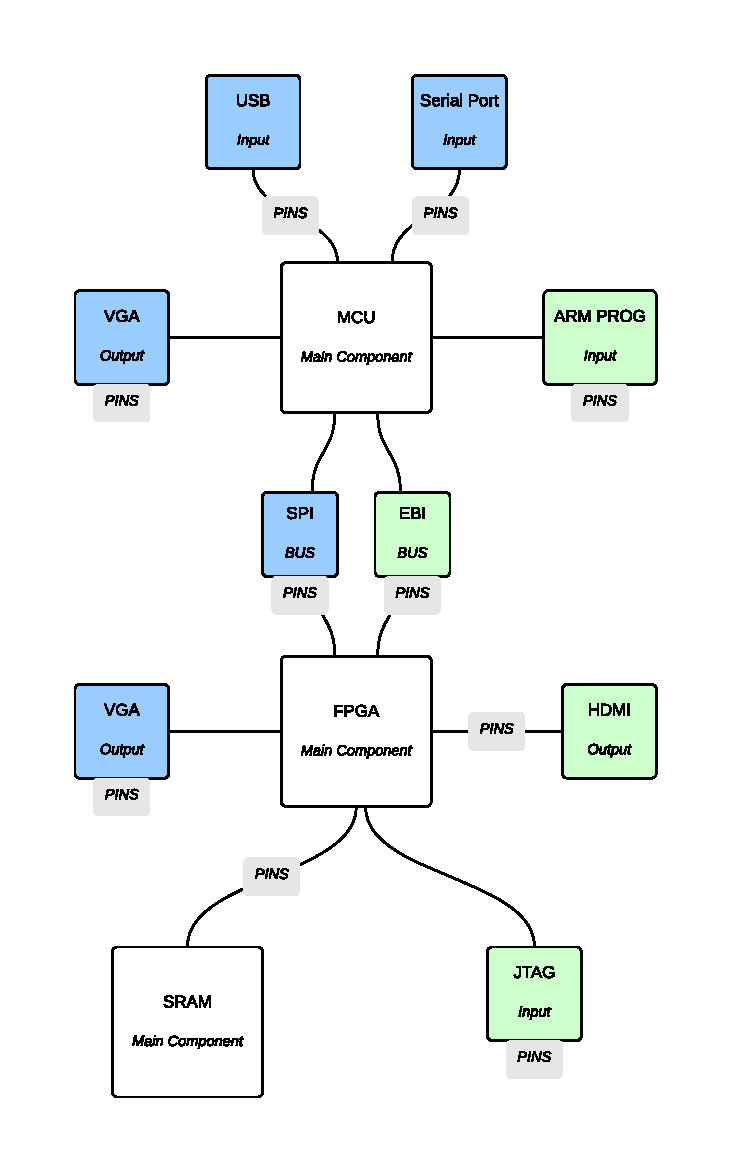
\includegraphics[width=0.65\textwidth]{../pcb/assets/pcb-overview.pdf}
    \label{fig:pcb-overview}
    \caption{Conceptual overview of the PCB. Green boxes are main solutions. Blue boxes are backup plans.
             Gray boxes labeled "PINS" means there are pins either on the wire itself, or that the box is pins.}
\end{figure}

These backup plans are in place to make sure the board will work, even if some parts are broken.
That way, each component can be connected to other sources than those on the board alone.
Because of this, the board is not optimized for the smallest size possible, but was rather made to optimize for highest possible chance of success.

\end{document}
